\documentclass[12pt,a4paper]{report}

%%% User pakcages

\usepackage[font=scriptsize]{caption} %small caption text
\usepackage{wrapfig}
\usepackage{afterpage}
\usepackage{parskip} % Disable US-type paragraph
\usepackage{amsfonts} % Math 
\usepackage{palatino} % Vektor fonts
\usepackage{mathptmx}
\usepackage[T1]{fontenc} 
\usepackage[utf8]{inputenc} %%\usepackage[utf8x]{inputenc} 
\usepackage{float}
\usepackage[danish]{babel} % Danish letters 
\usepackage{booktabs} % Nice tabels
\usepackage[pdftex]{graphicx} % Include graphics 
\usepackage{fancyhdr} % header & footer
\usepackage[hyphens]{url}
\usepackage[hidelinks, breaklinks]{hyperref} % Hyper link
\PassOptionsToPackage{hyphens}{url}\usepackage{hyperref}
\usepackage{titlesec}
\usepackage{xfrac}
\usepackage{listings} % Insert code
\usepackage[usenames,dvipsnames,svgnames,table]{xcolor}


\usepackage[backend=bibtex]{biblatex}
\bibliography{Kilder/kilder.bib}
\usepackage[left=2.5cm,right=2.5cm,top=2.5cm,bottom=2.5cm]{geometry} % Page margin
\usepackage{tabularx} % Table
\usepackage{marginnote}

\titleformat{\chapter}{\normalfont\huge\bfseries}{ \thechapter.}{20pt}{\huge}
\setcounter{section}{0}
\pagestyle{fancy}
\fancypagestyle{arabic}
{
    \fancyhf{}
    \setlength{\headheight}{15pt}
}

\renewcommand{\chaptermark}[1]{ \markboth{#1}{} }
\fancypagestyle{chp}{
  \fancyhf{}
  \rhead{\rightmark}%\colorbox{black}{\color{white}{\rightmark}}}
  \cfoot{\thepage}
}

\pagestyle{chp}

\title{Ground Handling}
\author{
    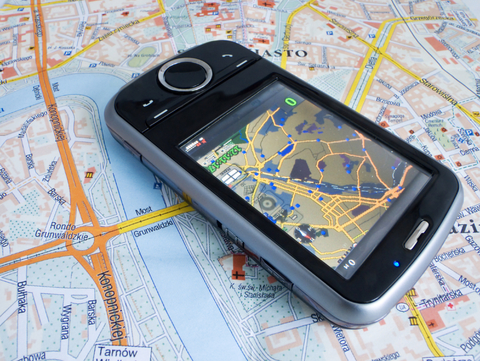
\includegraphics[width=14cm]{grafik/index} \\
        Kasper Ø. Helsted, Jens H. Stærmose, Christoffer C. Christensen, Christian H. Nielsen\\
        Kasper F. Christensen, Anders L. Matthiassen \& Josias Laugesen\\
}
\date{21 - 05 - 2014}

\definecolor{codecomment}{HTML}{383838}

\lstset{language=C,
    basicstyle=\ttfamily\scriptsize,
    keywordstyle=\color{Blue}\ttfamily,
    otherkeywords={WIDTH},
    keywords=[2]{__shared__},
    keywordstyle=[2]\color{orange}\ttfamily,
    stringstyle=\color{red}\ttfamily,
    commentstyle=\color{codecomment}\ttfamily,
    breaklines=true,
    numbers=left,
}

\begin{document}
    \maketitle
    \afterpage{\null\newpage}
    \pagenumbering{gobble}
    \clearpage  
    %Titlepage 
    \thispagestyle{empty}
\begin{titlepage}
	\setlength{\textwidth}{15cm}
	\noindent
	\begin{nopagebreak}
		{\samepage 
			\begin{tabular}{lr}
				\parbox{0.5\textwidth}{\raisebox{11mm}
					{
\includegraphics[height=1.2cm]{Grafik/aauLogoDa}}
				} &
				\parbox{0.5\textwidth}{
					\small
					\begin{tabular}{l}
						{\sf\small \textbf{Institute of Computer Science}}\\
						{\sf\small Strandvejen 12-14, 9000 Aalborg} \\
						{\sf\small Telephone 96 35 97 31} \\
						{\sf\small Fax 98 13 63 93} \\
						{\sf\small http://tnb.aau.dk}
					\end{tabular}
				}
			\end{tabular}
			
			\noindent
			\begin{tabular}{cc}
				\parbox{7cm}{
					\begin{description}
			
						\item {\bf Title:} 
			
							\textbf{Ground Handling}\\
						\item {\bf Project Period:}\\
			  				Spring Semester 2014\\
			 				\hspace{4cm}
						\item {\bf Project Group:}\\
							SW2-A418\\
			  				\hspace{4cm}
						\item {\bf Participants:}\\
							Kasper Østergaard Helsted\\
                            Jens Hegner Stærmose\\
                            Christoffer Carlé Christensen\\
                            Christian Heider Nielsen\\
                            Kasper Fuglsang Christensen\\
                            Anders Lykke Matthiassen\\
                            Josias Laugesen\\
							\hspace{2cm}
						\item {\bf Supervisor:}\\
							Ramin Sadre\\

						\item {\bf Copies:}\\ 10\\
						\item {\bf Page Numbers:}\\ 65\\
						\item {\bf Appendix:}\\ None\\
						\item {\bf Number and Type of Annexes:}\\ 14 pages, code\\
						\item {\bf Date of Completion:}\\ 21-05-2014\\
					\end{description}
					\vfill
				} &
				\parbox{7cm}{
					\vspace{.15cm}
					\hfill 
					\begin{tabular}{l}
						{\bf Abstract:}\bigskip \\
						\fbox{
							\parbox{6.5cm}{\smallskip
								{\vfill{\small \section* {Synopsis}

								\smallskip}}
							}
						}
  					\end{tabular}
  				}
			\end{tabular}
		}\\
		\\
		\noindent{\footnotesize\emph{The content of this report is freely accessible, but publication (with referencing) may only happen under agreement with the authors.}}
	\end{nopagebreak}
\end{titlepage}

    \afterpage{\null\newpage}
    \pagenumbering{gobble}
    \clearpage  
    \pagenumbering{roman}
    \chapter*{Forord}


    \renewcommand*\contentsname{Indholdsfortegnelse}
    \tableofcontents
    \thispagestyle{empty}
    \pagenumbering{arabic}
    \clearpage
    \setcounter{page}{1}
	
    \part{Produktudvikling}
    
    \printbibliography

\end{document}